Betrachtet werden die beiden Kurven, welche 9600 Samples lang und in Abbildung \ref{deconvolve:1d} dargestellt sind.
Beide Funktionen wurden mit einer diskreten Wavelet-Transformation mit Haar-Wavelet und 13 Level analysiert.
Die Transformation gibt also 13 verschiedene Sets an Koeffizienten zurück.
Auf Level 1 befinden sich die Koeffizienten, welche mit dem am höchsten aufgelösten Wavelet erhalten wurde.
Auf Level 13 sind demnach die Koeffizienten die von dem Wavelet mit der gröbsten Auflösung, bwz. grössten \glqq Wellenlänge \grqq{} herrühren.

Koeffizienten, welche die Transformation von $f(x)$ (Abbildung \ref{deconvolve:1d}) liefert, werden in dieser Arbeit $cf_k$ genannt.
Der Index $k\in[1:13]$ soll dabei das entsprechende Level der Koeffizienten sein.
Gleichermassen bezeichnet $cg_k$ die Koeffizienten der Funktion $g(x)$ auf Level $k$.

Kann nun eine Beziehung zwischen den Wavelet-Koeffizienten von $f(x)$ und $g(x)$ erkannt werden?
Die Hoffnung ist es, diesen Zusammenhang als Funktion zu formulieren welche $cf_k$ als Input nimmt und ein Set an Koeffizienten zurück gibt, welche den $cg_k$ ähnlich ist.
\begin{figure}[h]
\centering
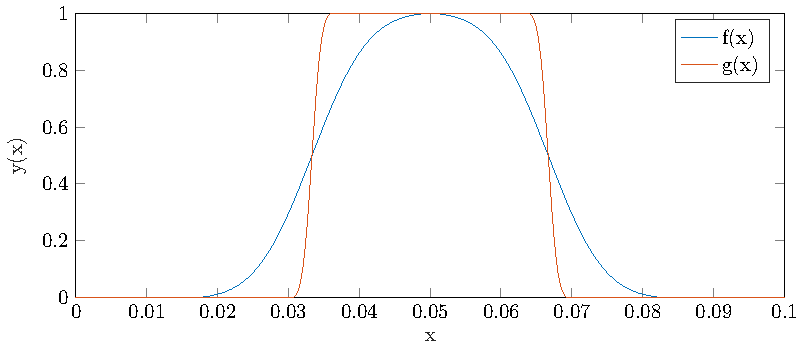
\includegraphics[width=0.9\textwidth]{./papers/deconvolve/pictures/1d.pdf}
\caption{Funktion\label{deconvolve:1d}}
\end{figure}

Die Rücktransformation mit den manipulierten $cf_k$ sollte dann eine Kurve liefern, welche derjenigen von $g(x)$ nahe kommt.
Bei Erfolg hätte man also eine Methode erarbeitet, welche aus der \glqq unscharfen\grqq{} $f(x)$ eine etwas \glqq schärfere\grqq{} Funktion $g(x)$ macht. 

\subsection{Koeffizienten manipulieren}
Abbildung \ref{deconvolve:level1} zeigt die Koeffizienten des ersten Levels der Funktionen $f(x)$ und $g(x)$ aus dem vorherigen Abschnitt.
\begin{figure}[h]
\centering
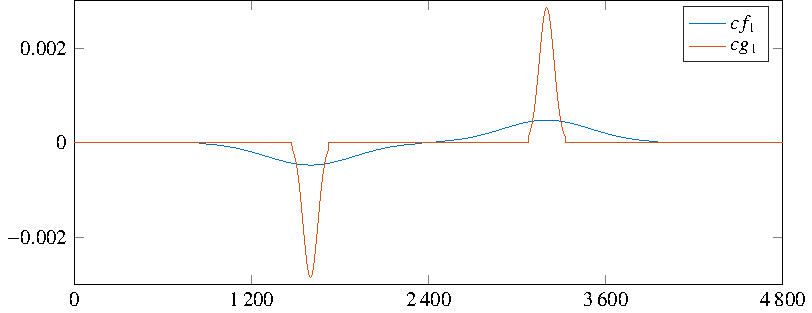
\includegraphics[width=0.9\textwidth]{./papers/deconvolve/pictures/level/level1.pdf}
\caption{Level 1 unverändert\label{deconvolve:level1}}
\end{figure}

Nun wird mit einer geeigneten Manipulation der Koeffizienten $cf_k$ versucht, die blauen Koeffizienten so anzupassen, bis sie den orangen möglichst ähnlich sind.
Es muss also eine Funktion gefunden werden, die als Input die Koeffizienten $cf_k$ nimmt und diese angenähert in die Koeffizienten $cg_k$ überführt.
Man erkennt klar, dass die $cf_1$, also die Koeffizienten des ersten Level der Funktion $f(x)$ unter einer gewissen Schwelle abgeschwächt und darüber überproportional verstärkt werden müssen.
$$\left( \frac{cf_k}{m}\right)^\alpha$$
ist hierfür ein vielversprechender Ansatz.
Der Parameter $m$ ist hierbei ebendiese Schwelle und mit $\alpha$ kann die Verstärkung bestimmt werden.
Wird aber $m$ sehr klein gewählt, so wird der Ausdruck in der Klammer grösser und mit der darauffolgenden Potenz $\alpha$ explodiert der Output dann förmlich.
Um dies auszugleichen muss nochmals mit $m$ multipliziert werden
$$m\cdot \left( \frac{cf_k}{m}\right)^\alpha.$$
Ein Problem stellen hier aber noch negative $cf_k$ dar. In diesem Fall kann nur mit ganzzahligen Potenzen gearbeitet werden, da man sonst komplexe Lösungen erhält, welche für diese Anwendung nicht brauchbar sind.
Um dies zu Umgehen muss nur der Betrag von $cf_k$ gebildet, und deren Vorzeichen aber noch mit der Signumfunktion mitgenommen werden.
Somit erhalten wir eine Funktion
\begin{align}
s(cf_k)=m\cdot \left(\frac{|cf_k|}{m}\right)^{\alpha}\cdot \text{sign}(cf_k), \qquad m,\alpha\in\mathbb{R}
\label{deconvolve:funktion}
\end{align}
als Beziehung zwischen dem \glqq unscharfen\grqq{} und \glqq scharfen\grqq{} Set an Koeffizienten.

Abbildung \ref{deconvolve:function} zeigt unsere Funktion aus \eqref{deconvolve:funktion} mit $m=0.2$, verschiedenen $\alpha$ und der Variable $cf_k\in[-1;1]$.
Gut erkennbar ist darin, wie mit dem Parameter $\alpha$ die Verstärkung justiert werden kann.
\begin{figure}[h]
\centering
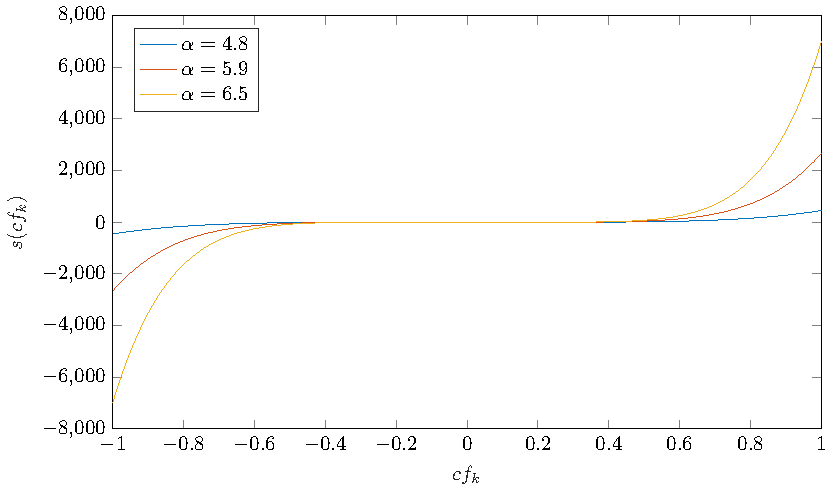
\includegraphics[width=0.9\textwidth]{./papers/deconvolve/pictures/function.pdf}
\caption{Funktion zur Schärfung\label{deconvolve:function}}
\end{figure}

Nun soll diese Funktion auf wenn möglich alle verschiedenen Level unserer Wavelet-Koeffizienten angewendet werden.
Für $m$ kann genau der Schnittpunkt zwischen den beiden Kurven in Abbildung \ref{deconvolve:level1} gewählt werden.
$\alpha$ wird dann so bestimmt, dass die Spitze der blauen Kurve nach der Manipulation mit derjenigen der orangen zusammenfällt.
\begin{figure}[h]
\centering
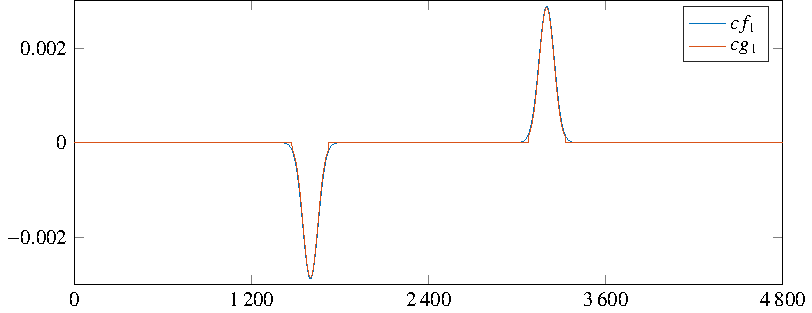
\includegraphics[width=0.9\textwidth]{./papers/deconvolve/pictures/level/level1_n.pdf}
\caption{Level 1 mit veränderten $cf_1$\label{deconvolve:level1_n}}
\end{figure}

Abbildung \ref{deconvolve:level1_n} zeigt die Funktion \eqref{deconvolve:funktion} wiederum auf das erste Level angewendet.
Der unterschied zwischen den beiden Kurven ist nur noch schwach erkennbar.

\subsection{Koeffizienten auf höheren Level}

Mit entsprechenden $m$ und $\alpha$ kann nun gleich auf den anderen Level vorgegangen werden.
Abbildung \ref{deconvolve:level5} zeigt Level 5 vor und nach der Koeffizientenmanipulation.
\begin{figure}[h]
\centering
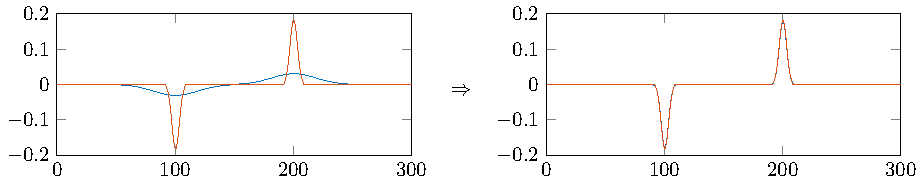
\includegraphics[width=0.9\textwidth]{./papers/deconvolve/pictures/level/level5.pdf}
\caption{Level 5 vorher und nachher\label{deconvolve:level5}}
\end{figure}

Auf diesem Level scheint alles noch wie erwünscht zu funktionieren.
Jeden Schritt höher kommen aber erwartungsgemäss weniger (halb so viele) Koeffizienten dazu.
Waren es im ersten noch 4800 sind es nun im fünften nur noch 300.
Auf dem Level 13 sind es dann nur noch zwei.
Deswegen wird es immer schwerer, die beiden Freiheitsgrade $m$ und $\alpha$ so zu wählen, dass noch eine Annäherung von $cf_k$ an $cg_k$ resultiert.
Mit dieser Beispielfunktion $f(x)$ war es möglich mit der Beziehung \eqref{deconvolve:funktion} bis auf das Level 12 eine Verbesserung zu erreichen.

\subsection{Ergebnis}
Abbildung \ref{deconvolve:result_1d} zeigt unsere ursprüngliche Kurve $f_1(x)$.
Dessen Wavelet-Koeffizienten $cf_k$ wurden dann mit der oben beschriebenen Methode bearbeitet, was nach der Rücktransformation zu $f_2(x)$ führt.
Verglichen mit $f_1(x)$, ist $f_2(x)$ deutlich näher an $g(x)$ gerückt.
\begin{figure}[h]
\centering
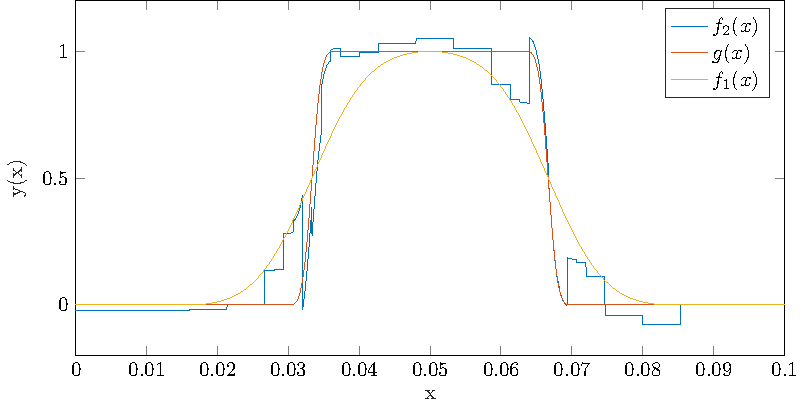
\includegraphics[width=0.9\textwidth]{./papers/deconvolve/pictures/result_1d.pdf}
\caption{Rücktransformation\label{deconvolve:result_1d}}
\end{figure}

In der Nähe des Randes hat sich die Steilheit tatsächlich vergrössert, allerdings sind weiter weg von diesem Rand zusätzliche Artefakte hinzugekommen.
Diese kommen von den Wavelets mit grösserer \glqq Wellenlänge \grqq{} bzw. höheren Level, welche schwerer zielführend zu manipulieren sind. Sie scheinen zu viel Einfluss zu haben.
